%%%%%%%%%%%%%%%%%%%%%%%%%%%%%%%%%%%%%%%%%%%%%%%%%%%%%%%%%%%%%%%%%
\chapter{INTRODUCTION}\label{Ch1}
%%%%%%%%%%%%%%%%%%%%%%%%%%%%%%%%%%%%%%%%%%%%%%%%%%%%%%%%%%%%%%%%%
% First level titles must be in capitals and bold (i.e. \textbf{1. INTRODUCTION)}, and placed on an odd page in the direction of reading.
\section{Cube Satellites}

A cube satellite, or cubesat, is a small  satellite made up of 10cm x 10cm x 10cm sized cubes\cite{cubesatspec}. One cube module is called 1 unit or 1U for short. Typically 1U has no more than 1.33kg of mass\cite{cubesatspec}\cite{herrera2016cubesat}. Depending on the mission, the size of the cubesat may vary from 1U to 27U's. Due to this fact a cubesat can either be classified as a nano satellite (1-10kg) or a micro satellite(10-100kg)\cite{konecny2004small}. A cube satellite can include several subsystems such as an on-board computer(OBC), electrical power system(EPS), atttitude determination and control system(ADCS), batteries and necessary payloads to perform its mission. Additionally, they can carry antennas to communicate with the ground station and solar cells to provide power to the subsystems and to recharge the batteries. 

The concept of cubesat was jointly developed by Stanford University and California Polytechnic University in 1999. It was designed as a tool to help students and engineers to develop necessary skills to design and operate satellites.  Majority of the cubesat launches have been originated by academic institutions. Even though the concept of a cubesat is created as a tool for educational purposes, recent advancements in electronics and sensor technology allow for more miniature components and expand the mission envelope for cubesats. Missions that could only be realized by large satellites such as high-resolution earth observation or complex scientific observations such as X-ray observation can now be performed by a cubesat. 

Due to their low cost and simplicity cubesats have become first ever satellites of some countries. Projects such as BIRDS by JAXA enables developed nations to partner with underdeveloped countries and produce their first space asset in the form of a cubesat\cite{pradhan2018birds}. 

As of 2022 more than 1600 cubesats have been launched into space\cite{Nanosats61online}. Vast majority of cubesats have been launched into LEO with very few of them are actually deployed into deep space. NASA's \textit{InSight} mission carried  MarCO-A and MarCO-B, first cubesats to leave LEO\cite{klesh2018marco}. There are plans to deploy cubesats into lunar orbit with upcoming Artemis missions as well\cite{tsay2015lunarcube}.
% \subsection{Propulsion systems used in cube satellites}
\subsection{Cube satellite research at ITU}
At Istanbul Technical University, any research related to cube satellites is handled by Space Systems Design and Testing Laboratory(SSDTL) operating under Eepartment of Aeronautics and Astronautics. Ever since its establishment in 2007, 7 cube satellites have been designed by SSDTL and 6 of them have been launced into space to perform variety of tasks such as earth observation, scientific missions or radio communication handling\cite{aslan2015integration}. Among the satellites launched into space is ITUpSAT-1, a 1U sized cubesat; first of its kind ever designed by Turkey\cite{aslanspace}. An image of flight model of ITUpSAT-1 is shown in figure \ref{fig:pSAT}.

\begin{figure}[ht]
    \centering
    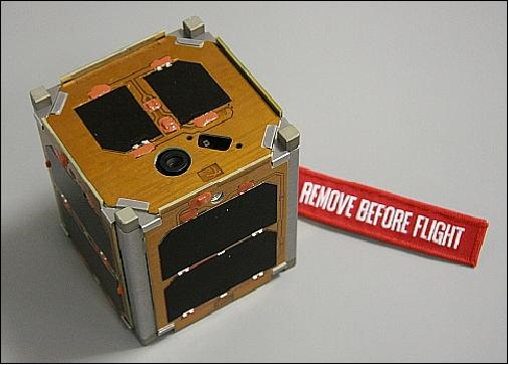
\includegraphics[scale=.9]{fig/ITUpSAT.png}
    \caption[1U sized cubesat ITUpSAT-1]{1U sized cubesat ITUpSAT-1\cite{aslanspace}}
    \label{fig:pSAT}
\end{figure}

In addition to satellites, various research have been performed into individual subsystems such as an interface board, OBC, an EPS and ADCS\cite{aslan2015integration}\cite{karabulut}[\textbf{INTERFACE KARTINA ATIF BUL}]. To date no work have been done regarding the propulsion systems for cube satellites. 

\section{Spacecraft Propulsion Systems}

A propulsion system is defined as a system that enables acceleration for a spacecraft. The contents of this section only includes propulsion systems that are used in space. Other systems such as launch vehicles are not included. 
Propulsion systems may be used to perform variety of tasks in space such as orbital maneuvering, station-keeping or attitude control. 
\par A propulsion system generates thrust, typically expressed in units of newtons(N) that in turn alters the spacecraft's velocity. Thrust is given as the change in momentum with respect to time\cite{goebel2008fundamentals}.

\begin{equation}
    T = \frac{d}{dt}(m_p v_{ex}) = \dot{m}_p v_{ex}
    \label{eq:thrust}
\end{equation}

where $m_p$ is the propellant mass, $v_{ex}$ is the exhaust velocity of the departing propellant and $\dot{m}_p$ is the flow rate of the propellant.


\par In order to examine the performance and propellant usage efficiency of the thruster the term "Specific Impulse" is used, denoted as $I_{sp}$. It is defined as the ratio of the generated thrust to the Earth weight of the flow rate of the propellant as shown in equation \ref{eq:Isp}.
\begin{equation}
    I_{sp} = \frac{T}{\dot{m}_p g}
    \label{eq:Isp}
\end{equation}

Substituting the expression of $\dot{m}_p$ from equation \ref{eq:thrust} into equation \ref{eq:Isp} gives;

\begin{equation}
    I_{sp} = \frac{v_{ex}}{g}
    \label{eq:IspVex}
\end{equation}

Using $v_{ex}$ for specific impulse calculations gives its unit in seconds (s). Higher specific impulse levels means more efficient propellant use. Ion thrusters, part of electric propulsion family, have specific impulse values around 3000 seconds but provide low thrust as opposed to chemical thrusters such as monopropellant thrusters which provide greater thrust at the cost of low specific impulse levels as low as 200 seconds\cite{tsay2009micro}\cite{lemmer2017propulsion}.


\par Based on their operating mechanism propulsion systems can be divided into two main groups as chemical and electric propulsion systems. This section includes general information regarding both types of systems to provide a basis for following sections. 
% Second level titles must be bold and the first letter of each word in the title must be capital (i.e. \textbf{2.1 Process Qualification Analysis}).

% \subsection{Third level title: Only first letter capital}

% Third and fourth level titles must be bold and only the first letter of the word the title begins with must be capital (i.e. \textbf{2.1.1 Process analysis using a histogram} or \textbf{3.1.1.2 Process analysis steps}).

% \subsection{Third level title}

% Third and fourth level titles must be bold and only the first letter of the word the title begins with must be capital (i.e. \textbf{2.1.1 Process analysis using a histogram} or \textbf{3.1.1.2 Process analysis steps}).



% \subsubsection{Fourth level title: Only first letter capital}

% Third and fourth level titles must be bold and only the first letter of the word the title begins with must be capital (i.e. \textbf{2.1.1 Process analysis using a histogram} or \textbf{3.1.1.2 Process analysis steps}).



% \subsubsection{Fourth level title: Only first letter capital}

% Third and fourth level titles must be bold and only the first letter of the word the title begins with must be capital (i.e. \textbf{2.1.1 Process analysis using a histogram} or \textbf{3.1.1.2 Process analysis steps}).

% %{\bf Fifth level title: No numbering after fourth level titles}
% \subsubsubsection{Fifth level title: No numbering after fourth level titles}
\subsection{Chemical propulsion systems}
Chemical propulsion systems exploit the energy in the molecular bonds of the propellant. When the propellant is ignited these molecular bonds are broken and energy is released. Thrust is generated when this hot, expanding propellant is ejected from the spacecraft.
\par Many cube satellites are launched into space as secondary payloads. Limitations of secondary payloads regarding the stored chemicals and combustion within the satellite pose serious challenges. Although there are several systems currently under development, so far no cube satellite with a chemical propulsion system have been launched into space\cite{lemmer2017propulsion}.
%  Depending on the type of the used propellant there are several types of chemical propulsion systems available: monopropellant, bi-propellant and solid rocket engines
% \subsubsection{Monopropellant}
% \subsubsection{Bi-propellant}
% \subsubsection{Solid rocket engines}
\subsection{Electric propulsion systems}
Electric propulsion systems provide thrust by accelerating their propellants. They use the on-board electrical power supply to generate thrust. Compared to chemical propulsion systems they produce less thrust and higher specific impulse\cite{Calik2011}. Due to their low thrust and high specific impulse output they are mainly used for space missions that require high $\Delta$V and propellant usage efficiency. Also due to the low thrust they are often subjected to long continuous use. EP systems can be further examined under three main groups: electrothermal, electrostatic and electromagnetic systems\cite{goebel2008fundamentals}.
\subsubsection{Electrothermal propulsion}

\subsubsubsection{Resistojet Thruster}
Resistojet thrusters constitute the simplest approach for an electric propulsion system. Compressed propellant, either in liquid or gas state, is fed into the nozzle of the thruster. Within the nozzle area is located a heating element. This heating element is usually just a simple resistor that produce ohmic heating due to current flow. As the propellant passes through the heating area it heats up and expands. This expanded gas is then ejected from the spacecraft to produce thrust. A schematic of a resistojet thruster is shown in figure \ref{fig:resistojet}

\begin{figure}[ht]
    \centering
    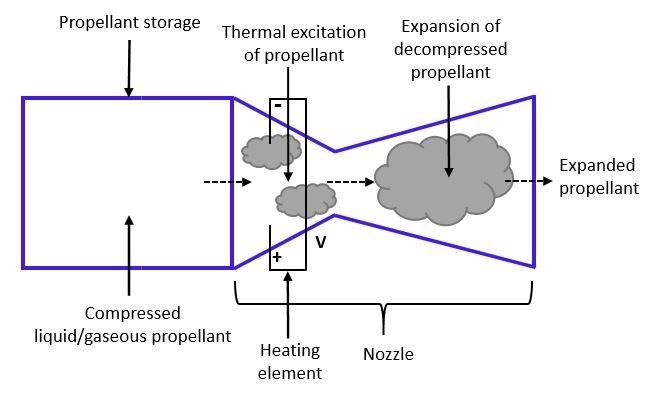
\includegraphics[scale=0.65]{fig/resistojet.png}
    \caption[Resistojet thruster schematic]{Resistojet thruster schematic\cite{tummala2017overview}}
    \label{fig:resistojet}
\end{figure}

Even though they have a considerable flight heritage on regular sized satellites none have flown into space on board a cube satellite so far\cite{lemmer2017propulsion}. Several companies have developed or in the process of developing resistojet thrusters. CubeSat High Impulse Propulsion System(CHIPS) designed and developed by CU Aerospace is stated to provide specific impulse of 76 s and thrust of 31 mN with 25W of power consumption\cite{hejmanowski2015cubesat}. Busek company has developed a micro resistojet thruster that can provide 150s specific impulse and 30 mN at 15W input power\cite{lemmer2017propulsion}. Both of these designs share similar sizes and occupy approximately 1U volume. 
\par Resistojet thrusters suffer from low efficiency obvious by their low specific impulse values. However considering their low power consumption and high thrust output they may be suitable for cubesat missions.

\subsubsubsection{Arcjet Thruster}

Similar to resistojets the aim of an arcjet thruster is to heat up the propellant and then eject the expanding propellant to create thrust. The method of heating up the propellant however, is different. Instead of a heating element an arcjet thruster consists of an anode, acentral cathode and injector. Prior the ignition high voltage, on the level of thousands of volts, is applied in between the cathode and anode. Ignition and arc forming occurs due to paschen-discharge\cite{wadhwa2006high} in the gap between the anode and cathode. Propellant injected into this gap is heated up and expanded. Expanded propellant is directed into the nozzle and thrust is generated. Working principle of an arcjet thruster is illustrated in figure \ref{fig:arcjet}

\begin{figure}[htb]
    \centering
    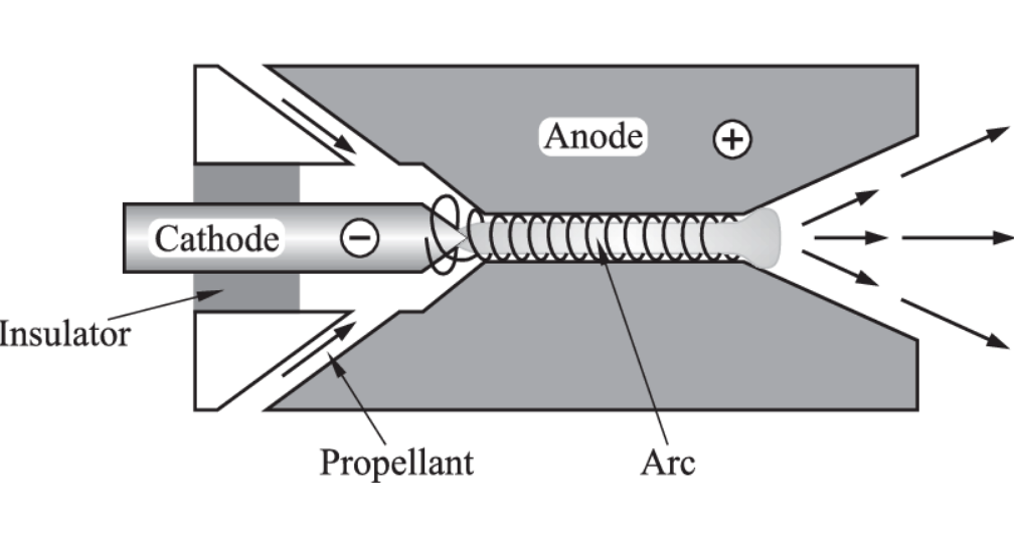
\includegraphics[scale=0.65]{fig/arcjet.png}
    \caption[Arcjet thruster schematic]{Arcjet thruster schematic\cite{bock2011electric}}
    \label{fig:arcjet}
\end{figure}

Plasma effects that occur because of the high current arc is neglectible since propellant is only weakly ionized. Specific impulse provided by the arcjets are recorded to be limited at approximately 700 s\cite{goebel2008fundamentals}.

\subsubsection{Electrostatic propulsion}
\subsubsubsection{Ion Thruster}
Ion thrusters, or sometimes called ion engines, utilize ions to create thrusts. These ions are supplied by the plasma generated and sustained within the thruster. In order to accelerate the ions a grid extraction system is used. This extraction system consists of two or three biased grids that create an electrostatic field. Any ion that encounters this electrostatic field is then ejected from the spacecraft. Depending on the mass of the used propellant ejected ions can reach speeds up to 1000 km/s\cite{goebel2008fundamentals}. They can provide $I_{sp}$ values up to 3500 s\cite{Calik2011}. Since spraying only ions from spacecraft will cause spacecraft be rapidly charged a neutralizer mechanism is needed to preserve the neutrality of the spacecraft.
\par There are three main types of ion thrusters in literature. First one is called Kaufman type thruster, also known as electron bombardment thruster, mainly studied in the United States, another one is RF ion thruster originated and predominantly studied in Germany and lastly Microwave or Electron-Cyclotron Resonance(ECR) thruster studied in Japan\cite{kokal2017design}\cite{OCW1964}\cite{Bumbarger}.
. Main difference between mentioned types of ion thrusters is their individual methods to create and sustain plasma. All subtypes of ion thrusters share the same ion acceleration mechanism. 

\par Working schematic of a Kaufman or electron bombardment ion thruster is shown in figure \ref{fig:kaufman}.

\begin{figure}[ht]
    \centering
    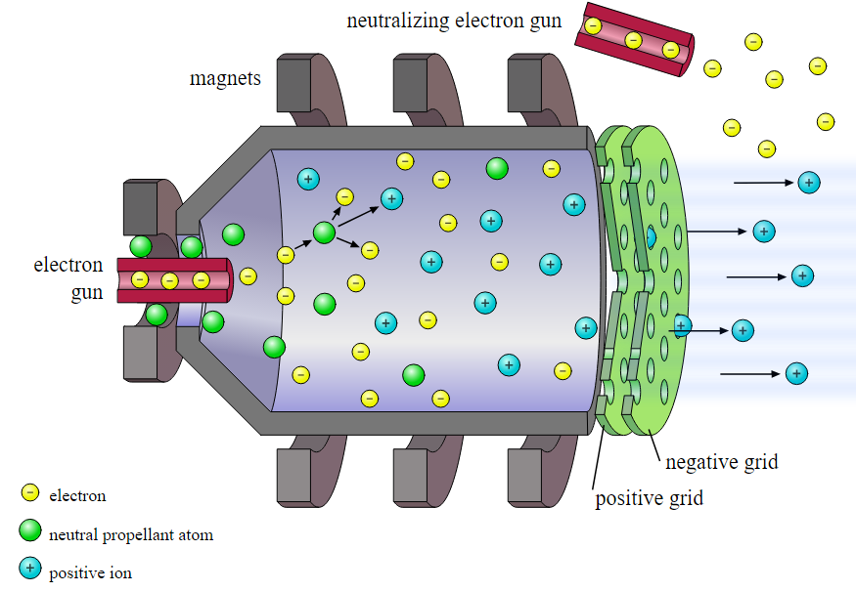
\includegraphics[scale=0.9]{fig/kaufman.png}
    \caption[Kaufman type ion thruster schematic]{Kaufman type ion thruster schematic\cite{kaufman}}
    \label{fig:kaufman}
\end{figure}

Electrons needed to ignite the plasma are pumped via an electron gun into the cylindirical discharge chamber. From same location neutral propellant is also fed into the chamber. Energetic electrons from electron gun collide with neutral propellant atoms and suffer elastic collisions. Through these collisions a valance electron from the neutral propellant atoms is ripped off. As a result an electron and an ion is obtained from the neutral atom in addition to the initial colliding electron. Energy acquired from the broken bond and presence of ions ignite the plasma and chain reaction resulting from increased density of electrons in the enviroment sustain the plasma\cite{goebel2008fundamentals}.
\par A pair of grids are located at the end of discharge chamber. Grid closer to the plasma is named as screen grid and is positively biased wheras the grid positioned away from the plasma is positively biased and named as acceleration grid. Electrostatic field created by the pair of grids accelerate the ions present in the plasma and create thrust\cite{kokal2017design}. Accelerated ions form an ion beam at the downstream of accelerator grids. Remaining electrons inside the plasma are drawn to walls which act as anodes. Magnets are used to create suitable magnetic fields to increase the amount of time electrons spend in the discharge chamber before evacuated to the anode and thus increase the chance of plasma ignition\cite{OCW1964}.
\par Same amount of electron density received at the anode walls of the thruster is injected into the extracted ion beam in order to keep the spacecraft neutral.

For RF ion thruster the plasma is formed by using a helical antenna wrapped around the discharge chamber. A diagram of such device is shown in figure \ref{fig:rfschematic}.

\begin{figure}[ht]
    \centering
    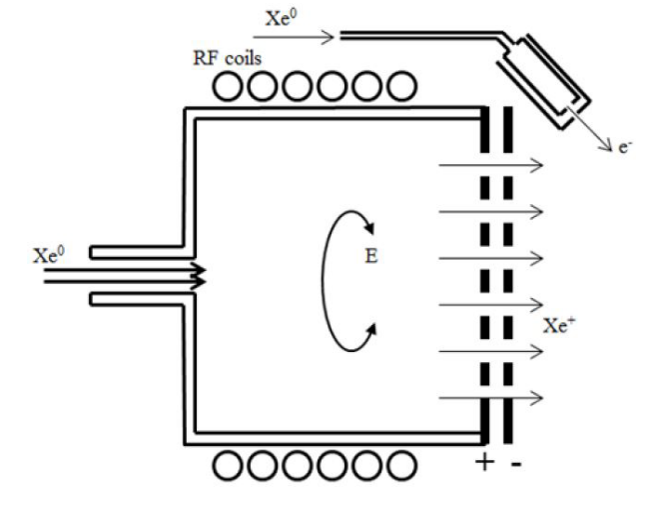
\includegraphics[scale=0.75]{fig/rfschematic.png}
    \caption[RF Ion Thruster Schematic]{RF Ion Thruster Schematic\cite{kokal2017design}}
    \label{fig:rfschematic}
\end{figure}

RF ion thrusters are cathodeless designs. Free electrons needed for plasma ignition can be retrieved from the neutralizer thruster chamber by reverse polarizing the grids. When an RF signal is broadcasted to the discharge chamber it acts as a solenoid and creates an axial magnetic field and perpendicular azimuthal electric field. Electrons inside the chamber start to display a tangential motion within the chamber under the influence of broadcasted signal and get energized. At this point a propellant is introduced to the discharge chamber. Electrons with high energy inside plasma collide with neutral propellant atoms and create a plasma. Depending on the power levels supplied by the RF antenna the resulting plasma can either be low density capacitively coupled plasma(CCP) or high density inductively coupled plasma(ICP). In CCP mode voltage from the helical coil is capacitively coupled to the chamber walls and create strong enough electric field to break down the propellant\cite{farnell2007performance}. During the ICP mode RF energy is coupled to the free electrons through magnetic induction\cite{Bumbarger}. RF signal is typically in the range of 1-13.56MHz\cite{mistoco2004development}.
The same two or three grid accelerator system used in Kaufman thrusters is used to accelerate and eject the ions from the device to create thrust. Main advantages of the RF ion thruster is that it utilizes a simple design and the helical coil is not in contact with plasma and thus have a longer life time. 

Electron-Cyclotron Resonance (ECR) thrusters utilize high frequcency (>1GHz) microwave(MW) signals to create a free floating plasma and heat the propellant. Working schematic is shown in figure \ref{fig:ecrschematic}.

\begin{figure}[ht]
    \centering
    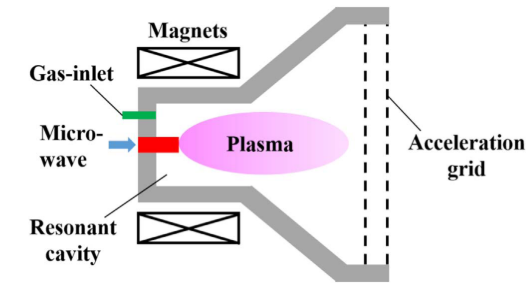
\includegraphics[scale=0.75]{fig/ecr.png}
    \caption[Schematic of ECR Thruster]{Schematic of ECR Thruster\cite{xiaogang2020heating}}
    \label{fig:ecrschematic}
\end{figure}

In a ECR microwave signals are broadcasted into the resonance cavity and a standing wave is formed. Free electrons present in the enviroment and propellant are coupled to the electric field and become ionized. These energetic electrons then collide with neutral propellant atoms to create a plasma similar to other types of ion thrusters. Once the plasma is ignited in the cavity region it can sustain itself by producing more free electrons and collisions. 

Main propellant type for ion thrusters are noble gasses such as Xenon, Krypton, Argon. Some non-noble gasses such as Mercury or Iodine have been used as well. Noble gasses are chemically inert and thus are safe to store. In addition they pose no risk of contamination for sensitive spacecraft surfaces such as solar panels or optics. Xenon have been predominantly used in electric propulsion purposes due to its high atomic mass (131amu) and higher thrust output but it requires more power to accelerate heavier Xenon when compared to other types of noble gasses. In addition Xenon is considerably expensive. Other types of noble gasses such as Argon or Krypton have gained popularity. With atomic masses of 39 amu and 83 amu for Argon and Krypton respectively they provide less thrust than Xenon but their wide availabilty make them more appealing\cite{Calik2011}. 




\subsubsubsection{Hall Thruster}
Hall thrusters, like ion engines, use ions to create thrusts. They employ magnetic circuits to trap electrons and collide trapped electrons with neutral propellant to create ions. Created ions are expelled from the thruster by utilizing the electric field created by the same magnetic circuit used to trap the electrons. A working schematic of a typical hall thruster is shown in figure \ref{fig:HET}.

\begin{figure}[ht]
    \centering
    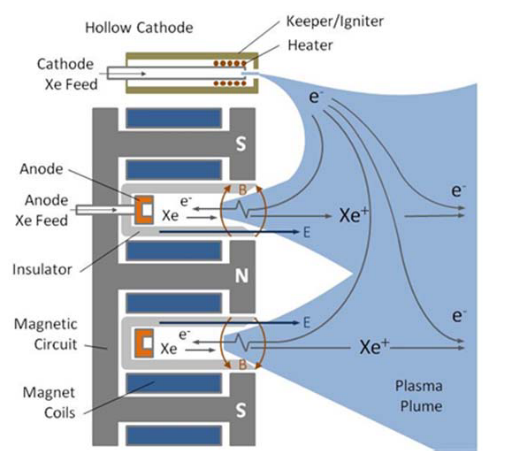
\includegraphics[scale=0.75]{fig/HET.png}
    \caption[Schematic of Hall Effect Thruster]{Schematic of Hall Effect Thruster\cite{szabo2020one}}
    \label{fig:HET}
\end{figure}

An electron source, in the case of figure \ref{fig:HET} a hollow cathode, is used to provide electrons. An anode is used to attract the electrons to the annular channel within the thruster. Once electrons are within the channel they are trapped due to radial magnetic fields created by specifically located magnetic circuits. Electrons inside the channel begin to exhibit tangential motion around the thruster axial axis. During this motion they incur a current called Hall current, hence the thruster's name. A neutral propellant is injected into the channel. Propellant atoms collide with energetic electrons inside channel and are ionized. Created ions are accelerated and subsequently ejected from the thruster by an axial electric field, perpendicular to the magnetic field created by the magnetic circuit. Some of the electrons originated from the cathode is used to neutralize the created ion beam. 

\par They contain a simple design compared to ion engines but magnetic and electric fields needs to be optimized to provide an efficient operation. Their $I_{sp}$ and efficiency values are somewhat less than other types of electorstatic propulsion systems but their thrust levels are significantly higher\cite{goebel2008fundamentals}. 

% \subsubsubsection{Field Emmission Electric Propulsion(FEEP) Thruster}


\subsubsection{Electromagnetic propulsion}

\subsubsubsection{Pulsed Plasma Thruster (PPT)}
Capacitors and spark igniters are used to create a discharge through a series of impulse bits. Solid, liquid or gas propellant can be used. If the used propellant is solid then this discharge ablates and removes small parts of the propellant. Same discharge also partially ionizes the propellant. Ionized propellant is then accelerated by Lorentz forces\cite{lemmer2017propulsion}. 
\par PTFE is traditionally used as solid propellant\cite{yost2021state}. Thrust levels are limited to the frequency of the charged capacitor. Spark igniter can limit the lifetime of the thruster. Their advantage is low power use. They can generate moderately high $I_{sp}$ values up to 800 s with 80$\mu$N with only 10W of power\cite{Calik2011}.

\subsubsubsection{Magnetoplasmadynamic (MPD) Thruster}
In MPD thrusters a propellant is ionized by using arcs generated by high currents. Ionized propellant is accelerated by electromagnetic forces such as Lorentz force to generate thrust. Since Lorentz force $J\times B$, where J is the current density and B is the magnetic flux density, utilize both current and magnetic field MDP's require greater power compared to other types of electric propulsion systems. At the same time they provide higher thrust (>1N) and higher $I_{sp}$ values (>5000 s)\cite{zheng2021integrated}. Working schematic of an MPD is shown in figure \ref{fig:MPD}

\begin{figure}[ht]
    \centering
    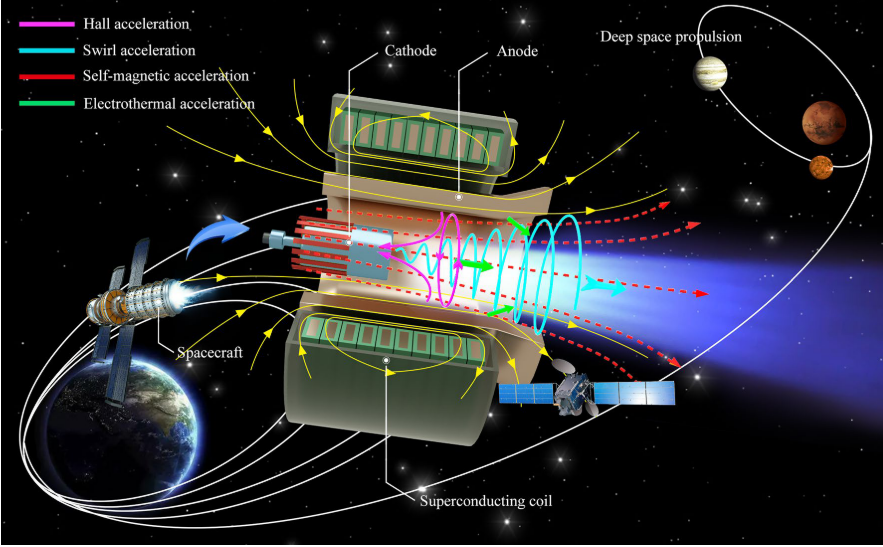
\includegraphics[scale=0.6]{fig/MPD.png}
    \caption[Working principle of a MPD thruster]{Working principle of a MPD thruster\cite{zheng2021integrated}}
    \label{fig:MPD}
\end{figure}

\newpage

\section{Thesis Purpose and Overview}\label{purposeofthesis}
Cube satellites offer very limited power budgets and volume limitations due to their small sizes. For an electric propulsion system to work properly it should be both compact and power efficient. Considering these factors for this thesis study an RF ion thruster is selected to be built. [\textbf{DÜZELT}]
RF ion thrusters do not include complex parts such as an electron source or magnets to confine the plasma. Their design simply consists of a plasma generator; an RF antenna wrapped around a discharge chamber and a pair of biased grids. Regardless of their simplicity they offer the highest $I_{sp}$ among the electric propulsion systems and are renowned for their scalability\cite{tsay2016maturation}. 
Another reason for RF ion thruster choice is the significant accumulation of know-how regarding their structure and testing at Bogazici University Space Technologies Laboratory(BUSTLab). Testing equipment within the BUSTLab such as the vacuum chamber, DC power sources, matching network tuner and RF signal generator are best suited for RF ion thruster operations\cite{yavuz2013prototype}.  
